% Vietnamese translation for OI Public Library
% Source-PDF: IOI中国国家候选队论文/2007/day2/7.胡伯涛《最小割模型在信息学竞赛中的应用》.pdf
\documentclass[11pt]{article}
\usepackage{oipl-vn}

\usepackage{array}
\usepackage{tikz}
\usetikzlibrary{arrows.meta,calc,decorations.pathmorphing,decorations.pathreplacing,fit,matrix,positioning,shapes.geometric}
\renewcommand{\figurename}{Hình}

\newcommand{\Oh}{\mathcal{O}}
\newcommand{\INF}{\infty}
\newcommand{\xor}{\mathbin{\mathrm{xor}}}
\newcommand{\R}{\mathbb{R}}

\tikzset{
  flow node/.style={circle,draw,minimum size=7mm,inner sep=0pt,font=\small},
  flow edge/.style={-{Stealth[length=2mm]},thick},
  flow weak/.style={flow edge,dashed},
  cut edge/.style={flow edge,red!75!black,line width=1.2pt},
  chosen edge/.style={red!75!black,line width=1.4pt},
  blue path/.style={blue!70!black,line width=1.1pt,dashed,-{Stealth[length=2mm]}},
  grid cell/.style={draw,minimum size=7mm,inner sep=0pt,font=\scriptsize},
}

\title{Mô hình cắt nhỏ nhất và ứng dụng trong thi tin học}
\author{Hu Botao (Amber)\\Trường Trung học số 1 Phúc Châu}
\date{2007}

\begin{document}
\maketitle

\origtitle{Applications of Minimum Cut Model in Informatics}
\sourcepath{IOI China candidate team papers / 2007 / day 2 / Hu Botao}

\begin{abstract}
Bài viết nghiên cứu định nghĩa, tính chất và các kiến thức mở rộng liên quan
tới mô hình cắt nhỏ nhất. Trọng tâm là bốn hướng ứng dụng: ứng dụng trực tiếp
từ định nghĩa; đồ thị đóng trọng số lớn nhất; đồ thị con mật độ lớn nhất; và
tập phủ đỉnh trọng số nhỏ nhất cùng tập độc lập đỉnh trọng số lớn nhất trong
đồ thị hai phía. Qua đó bài viết trình bày và phân tích cách dựng đồ thị cũng
như lối tư duy đặc thù của mô hình cắt nhỏ nhất, rồi tổng kết các phương pháp
và kỹ thuật thường dùng khi áp dụng mô hình này.
\end{abstract}

\paragraph{Từ khóa.}
Luồng mạng; luồng cực đại; cắt nhỏ nhất; đồ thị đóng trọng số lớn nhất; đồ
thị con mật độ lớn nhất; tập phủ đỉnh trọng số nhỏ nhất trong đồ thị hai phía;
tập độc lập đỉnh trọng số lớn nhất trong đồ thị hai phía.

\begin{abstract}
This article studies the definition, properties and related extensions of the
minimum-cut model. It focuses on direct applications, maximum weight closure,
maximum density subgraph, and weighted vertex cover/independent set in
bipartite graphs, emphasizing construction methods and common transformation
patterns.
\end{abstract}

\tableofcontents

\section{Lời nói đầu}

Cắt nhỏ nhất là bài toán đối ngẫu của luồng cực đại. Trong quá trình mô hình
hóa thực tế, nó thường kém trực quan hơn luồng cực đại; mô hình cũng hay ẩn
sâu trong đề bài, nên không dễ tìm ra cách dựng mạng. Bài viết này tập trung
vào ứng dụng thực tế của mô hình cắt nhỏ nhất, trình bày các cách dựng đồ thị
tinh tế và lối tư duy riêng của nó, đồng thời tổng kết phương pháp và kỹ thuật
chung khi xây dựng loại mô hình này.

Phần 1 giới thiệu kiến thức nền về luồng mạng và quy hoạch phân thức, làm cơ
sở cho các phần sau. Riêng quy hoạch phân thức được mở rộng từ dạng \(0\)-\(1\)
trong tài liệu của Liu và Huang sang dạng tổng quát hơn. Phần 2 dùng hai ví
dụ tương đối đơn giản để minh họa cách ứng dụng trực tiếp cắt nhỏ nhất từ
định nghĩa. Phần 3 trình bày mô hình đồ thị đóng trọng số lớn nhất và cách
giải bằng cắt nhỏ nhất, trong đó phần chứng minh cách dựng là trọng tâm. Phần
4 trình bày mô hình đồ thị con mật độ lớn nhất: trước hết quy về đồ thị đóng
trọng số lớn nhất, sau đó đưa ra một cách dùng cắt nhỏ nhất hiệu quả hơn, rồi
mở rộng tới đồ thị có trọng số cạnh và đồ thị có cả trọng số đỉnh lẫn cạnh.
Phần 5 trình bày tập phủ đỉnh trọng số nhỏ nhất và tập độc lập đỉnh trọng số
lớn nhất trong đồ thị hai phía. Phần 6 tổng kết một số hướng suy nghĩ khi dùng
mô hình cắt nhỏ nhất.

Bài viết đặt trọng tâm vào phân tích ý tưởng, không phải chỉ là giới thiệu
thuật toán. Vì vậy, nhiều dung lượng được dùng để mô tả quá trình biến đổi tư
duy. Mạch phân tích về cơ bản đi theo các bước trong bảng ``How to Solve It''
của George Polya. Sau mỗi phân tích, bài viết đưa ra chứng minh ngắn gọn để
kết tinh quá trình suy luận.

\section{Kiến thức chuẩn bị}

\subsection{Mạng và luồng}

\term{Mạng luồng} \(G=(V,E)\), gọi tắt là mạng, là một đồ thị có hướng. Mỗi
cạnh \((u,v)\in E\) có sức chứa không âm \(c(u,v)\ge 0\); nếu
\((u,v)\notin E\) thì quy ước \(c(u,v)=0\). Trong mạng có hai đỉnh đặc biệt:
nguồn \(s\) và đích \(t\).

Một \term{luồng} trên mạng \(G\) là hàm thực \(f:V\times V\to\R\) thỏa ba
tính chất sau:
\begin{enumerate}
  \item Ràng buộc sức chứa: với mọi \(u,v\in V\), \(f(u,v)\le c(u,v)\).
  \item Phản đối xứng: với mọi \(u,v\in V\), \(f(u,v)=-f(v,u)\).
  \item Bảo toàn luồng: với mọi \(u\in V-\{s,t\}\),
  \[
    \sum_{v\in V} f(u,v)=0.
  \]
\end{enumerate}
Giá trị của luồng là
\[
  |f|=\sum_{v\in V} f(s,v). \tag{1.1}
\]
Luồng cực đại là luồng có giá trị lớn nhất trong mạng.

Để tiện ký hiệu, nếu đối số của \(f\) là tập đỉnh thì hiểu là lấy tổng trên
mọi phần tử của tập đó:
\[
  f(X,Y)=\sum_{u\in X}\sum_{v\in Y} f(u,v).
\]

\paragraph{Bổ đề 1.1 (các phép tính cơ bản của luồng).}
Nếu \(f\) là một luồng trên \(G=(V,E)\), thì:
\[
  f(X,X)=0,\qquad
  f(X,Y)=-f(Y,X),
\]
và nếu \(X\cap Y=\varnothing\) thì
\[
  f(X\cup Y,Z)=f(X,Z)+f(Y,Z).
\]

\subsection{Mạng dư và đường tăng}

Mạng dư, đường tăng và cắt là ba khái niệm nền cho định lý luồng cực đại cắt
nhỏ nhất. Cho mạng \(G=(V,E)\) và một luồng \(f\). Với mỗi cặp đỉnh, sức chứa
dư được định nghĩa là
\[
  c_f(u,v)=c(u,v)-f(u,v). \tag{1.2}
\]
Mạng dư là \(G_f=(V,E_f)\), trong đó
\[
  E_f=\{(u,v)\in V\times V\mid c_f(u,v)>0\}.
\]
Nói trực quan, mạng dư gồm các cạnh còn có thể tiếp nhận thêm luồng.

\paragraph{Bổ đề 1.2 (mạng dư và mạng gốc).}
Nếu \(f\) là một luồng trong \(G\), còn \(f'\) là một luồng trong mạng dư
\(G_f\), thì \(f+f'\) vẫn là một luồng trong \(G\).

\term{Đường tăng} \(p\) là một đường đơn từ \(s\) tới \(t\) trong mạng dư
\(G_f\). Sức chứa dư của đường này là
\[
  c_f(p)=\min\{c_f(u,v)\mid (u,v)\in p\}>0.
\]
Định nghĩa luồng \(f_p\) trên đường tăng:
\[
  f_p(u,v)=
  \begin{cases}
    c_f(p), & (u,v)\in p,\\
    -c_f(p), & (v,u)\in p,\\
    0, & \text{trường hợp khác.}
  \end{cases}
\]

\paragraph{Bổ đề 1.3 (khả năng tăng luồng).}
Với mạng \(G=(V,E)\), luồng \(f\) và đường tăng \(p\), hàm \(f+f_p\) vẫn là
một luồng trong \(G\), và có giá trị lớn hơn \(f\).

\subsection{Luồng cực đại và cắt nhỏ nhất}

\term{Cắt} \([S,T]\) của mạng \(G=(V,E)\) là một phân hoạch \(V=S\cup T\),
\(S\cap T=\varnothing\), sao cho \(s\in S\) và \(t\in T\). Ký hiệu \([S,T]\)
cũng chỉ tập cạnh
\[
  \{(u,v)\in E\mid u\in S,\ v\in T\}.
\]
Luồng ròng qua cắt là \(f(S,T)\), còn sức chứa của cắt là
\[
  c[S,T]=c(S,T)=\sum_{u\in S}\sum_{v\in T} c(u,v).
\]
Cắt nhỏ nhất là cắt có sức chứa nhỏ nhất.

Một điểm dễ nhầm là cạnh từ \(T\) về \(S\) có đóng góp âm vào luồng ròng
\(f(S,T)\), nhưng không được tính vào sức chứa \(c[S,T]\). Sức chứa cắt chỉ
tính các cạnh đi từ phía nguồn sang phía đích.

\begin{figure}[htbp]
\centering
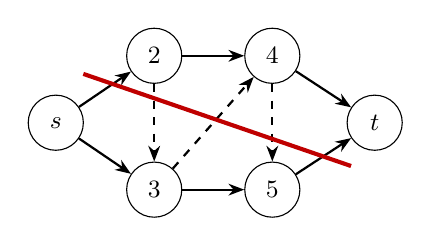
\begin{tikzpicture}[x=1cm,y=1cm]
  \node[flow node] (s) at (0,0) {\(s\)};
  \node[flow node] (n2) at (1.25,0.85) {2};
  \node[flow node] (n3) at (1.25,-0.85) {3};
  \node[flow node] (n4) at (2.75,0.85) {4};
  \node[flow node] (n5) at (2.75,-0.85) {5};
  \node[flow node] (t) at (4.05,0) {\(t\)};
  \draw[flow edge] (s) -- (n2);
  \draw[flow edge] (s) -- (n3);
  \draw[flow edge] (n2) -- (n4);
  \draw[flow edge] (n3) -- (n5);
  \draw[flow edge] (n4) -- (t);
  \draw[flow edge] (n5) -- (t);
  \draw[flow weak] (n2) -- (n3);
  \draw[flow weak] (n3) -- (n4);
  \draw[flow weak] (n4) -- (n5);
  \draw[red!75!black,line width=1.5pt] (0.35,0.62) -- (3.75,-0.55);
\end{tikzpicture}
\caption{Ví dụ cắt nhỏ nhất trong nguồn: các đỉnh dưới đường đỏ thuộc \(S\);
các đỉnh còn lại thuộc \(T\).}
\end{figure}

\paragraph{Bổ đề 1.4 (quan hệ giữa cắt và luồng).}
Với mọi luồng \(f\) và mọi cắt \([S,T]\) của \(G\), ta có
\[
  f(S,T)=|f|.
\]
\emph{Chứng minh.}
\[
\begin{aligned}
f(S,T)&=f(S,V)-f(S,S)\\
      &=f(S,V)\\
      &=f(\{s\},V)+f(S-\{s\},V)\\
      &=f(s,V)=|f|.
\end{aligned}
\]
Dòng cuối dùng tính bảo toàn luồng trên các đỉnh trong \(S-\{s\}\).

\paragraph{Hệ quả 1.5 (tính chất đối ngẫu).}
Với mọi luồng \(f\) và mọi cắt \([S,T]\), luôn có
\[
  |f|\le c[S,T].
\]
Thật vậy,
\[
  |f|=f(S,T)=\sum_{u\in S}\sum_{v\in T} f(u,v)
  \le \sum_{u\in S}\sum_{v\in T} c(u,v)=c[S,T].
\]

\paragraph{Định lý 1.6 (luồng cực đại cắt nhỏ nhất).}
Cho luồng \(f\) trong mạng \(G=(V,E)\) có nguồn \(s\) và đích \(t\). Ba điều
kiện sau tương đương:
\begin{enumerate}
  \item \(f\) là một luồng cực đại của \(G\);
  \item mạng dư \(G_f\) không chứa đường tăng;
  \item tồn tại một cắt \([S,T]\) của \(G\) sao cho \(|f|=c[S,T]\).
\end{enumerate}
\emph{Chứng minh.}
Nếu \(f\) cực đại mà \(G_f\) còn đường tăng \(p\), theo Bổ đề 1.3 có thể tăng
luồng, mâu thuẫn. Ngược lại, nếu \(G_f\) không có đường từ \(s\) tới \(t\),
đặt
\[
  S=\{v\in V\mid \text{có đường từ }s\text{ tới }v\text{ trong }G_f\},\qquad
  T=V-S.
\]
Khi đó \(s\in S\), \(t\in T\). Với mọi \(u\in S, v\in T\), không thể có
sức chứa dư dương trên cạnh \((u,v)\), nên \(f(u,v)=c(u,v)\). Bởi Bổ đề 1.4,
\(|f|=f(S,T)=c[S,T]\). Cuối cùng, nếu \(|f|=c[S,T]\) với một cắt nào đó thì
Hệ quả 1.5 cho thấy không luồng nào có giá trị lớn hơn \(f\).

\subsection{Thuật toán tìm cắt nhỏ nhất}

Từ định lý trên, muốn tìm một cắt nhỏ nhất ta làm hai bước. Trước hết tìm
luồng cực đại \(f\). Sau đó xét mạng dư \(G_f\), duyệt DFS hoặc BFS từ nguồn
\(s\); tập các đỉnh tới được là \(S\), phần còn lại là \(T\). Cắt \([S,T]\) là
một cắt nhỏ nhất.

Cần lưu ý: mọi cạnh trong cắt nhỏ nhất đều bão hòa, nhưng không phải mọi cạnh
bão hòa đều thuộc cắt nhỏ nhất. Trong những mạng đặc biệt, chẳng hạn mạng
dựng từ đồ thị hai phía với các cạnh giữa hai phía có sức chứa rất lớn, việc
chỉ nhìn các cạnh bão hòa kề nguồn hoặc kề đích là sai. Phải duyệt trên mạng
dư sau khi có luồng cực đại; một số đỉnh nhìn như đã bị tách khỏi nguồn vẫn
có thể tới được qua cạnh ngược trong mạng dư.

\begin{figure}[htbp]
\centering
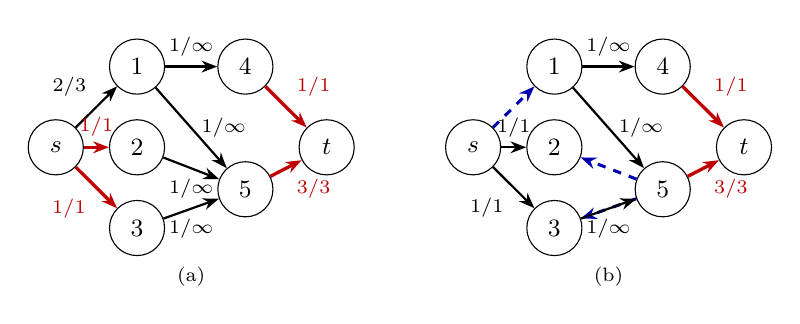
\begin{tikzpicture}[x=0.86cm,y=0.82cm, every node/.style={font=\scriptsize}]
  \begin{scope}
    \node[flow node] (s) at (0,0) {\(s\)};
    \node[flow node] (a1) at (1.2,1.25) {1};
    \node[flow node] (a2) at (1.2,0) {2};
    \node[flow node] (a3) at (1.2,-1.25) {3};
    \node[flow node] (a4) at (2.8,1.25) {4};
    \node[flow node] (a5) at (2.8,-0.65) {5};
    \node[flow node] (t) at (4.0,0) {\(t\)};
    \draw[flow edge] (s) -- node[above left]{\(2/3\)} (a1);
    \draw[cut edge] (s) -- node[above]{\(1/1\)} (a2);
    \draw[cut edge] (s) -- node[below left]{\(1/1\)} (a3);
    \draw[flow edge] (a1) -- node[above]{\(1/\infty\)} (a4);
    \draw[flow edge] (a1) -- node[right]{\(1/\infty\)} (a5);
    \draw[flow edge] (a2) -- node[below]{\(1/\infty\)} (a5);
    \draw[flow edge] (a3) -- node[below]{\(1/\infty\)} (a5);
    \draw[cut edge] (a4) -- node[above right]{\(1/1\)} (t);
    \draw[cut edge] (a5) -- node[below right]{\(3/3\)} (t);
    \node at (2,-2.0) {(a)};
  \end{scope}
  \begin{scope}[xshift=5.3cm]
    \node[flow node] (s) at (0,0) {\(s\)};
    \node[flow node] (b1) at (1.2,1.25) {1};
    \node[flow node] (b2) at (1.2,0) {2};
    \node[flow node] (b3) at (1.2,-1.25) {3};
    \node[flow node] (b4) at (2.8,1.25) {4};
    \node[flow node] (b5) at (2.8,-0.65) {5};
    \node[flow node] (t) at (4.0,0) {\(t\)};
    \draw[blue path] (s) -- (b1);
    \draw[flow edge] (s) -- node[above]{\(1/1\)} (b2);
    \draw[flow edge] (s) -- node[below left]{\(1/1\)} (b3);
    \draw[flow edge] (b1) -- node[above]{\(1/\infty\)} (b4);
    \draw[flow edge] (b1) -- node[right]{\(1/\infty\)} (b5);
    \draw[blue path] (b5) -- (b2);
    \draw[blue path] (b5) -- (b3);
    \draw[flow edge] (b3) -- node[below]{\(1/\infty\)} (b5);
    \draw[cut edge] (b4) -- node[above right]{\(1/1\)} (t);
    \draw[cut edge] (b5) -- node[below right]{\(3/3\)} (t);
    \node at (2,-2.0) {(b)};
  \end{scope}
\end{tikzpicture}
\caption{Ví dụ đồ thị hai phía: hình (a) minh họa cách chọn sai
chỉ từ cạnh bão hòa; hình (b) cho thấy các đường dư màu xanh khiến cắt đúng
phải lấy các cạnh đỏ phía đích.}
\end{figure}

\subsection{Một số thuật toán luồng cực đại}

Bài viết này không đi sâu vào thuật toán luồng cực đại, nhưng cắt nhỏ nhất
thường được tìm thông qua luồng cực đại. Với \(n=|V|\), \(m=|E|\), và \(U\)
là sức chứa lớn nhất, các thuật toán thường gặp gồm:

\begin{center}
\begin{tabular}{>{\raggedright\arraybackslash}p{0.33\linewidth}
                >{\centering\arraybackslash}p{0.17\linewidth}
                >{\raggedright\arraybackslash}p{0.42\linewidth}}
\hline
Thuật toán & Độ phức tạp & Ý chính\\
\hline
Ford--Fulkerson tổng quát & \(\Oh(nmU)\) &
Mỗi lần tìm tùy ý một đường tăng trong mạng dư.\\
Tăng luồng theo co giãn sức chứa & \(\Oh(nm\log U)\) &
Ưu tiên các đường có khả năng tăng lớn theo từng ngưỡng sức chứa.\\
Edmonds--Karp & \(\Oh(nm^2)\) &
Mỗi lần dùng BFS để tìm đường tăng ngắn nhất theo số cạnh.\\
Dinic & \(\Oh(n^2m)\) &
Dùng BFS tạo mức, rồi nhiều lần DFS trên đồ thị mức để tìm luồng chặn.\\
Preflow-push tổng quát & \(\Oh(n^2m)\) &
Duy trì tiền luồng, lặp các thao tác đẩy và đổi nhãn trên đỉnh hoạt động.\\
FIFO preflow-push & \(\Oh(n^3)\) &
Duy trì đỉnh hoạt động bằng hàng đợi FIFO.\\
Highest-label preflow-push & \(\Oh(n^2\sqrt m)\) hoặc chặn gần kề tùy biến thể &
Luôn xử lý đỉnh hoạt động có nhãn cao nhất.\\
\hline
\end{tabular}
\end{center}

Trong lập trình thi đấu, thuật toán tăng đường thường có hiệu quả thực tế tốt
vì số lần tăng luồng trên nhiều mạng không quá lớn. Preflow-push có chặn lý
thuyết mạnh, nhưng trên đồ thị thưa đôi khi không nhanh bằng các thuật toán
tăng đường được cài đặt tốt. Trong các phần sau, độ phức tạp của bước này
được viết gọn là \(\Oh(\operatorname{MaxFlow}(N))\).

\subsection{Quy hoạch phân thức}

Dạng tổng quát của quy hoạch phân thức là
\[
  \text{Minimize }\lambda=f(x)=\frac{a(x)}{b(x)}\quad (x\in S),
  \qquad b(x)>0.
\]
Ở đây \(x\) là vector nghiệm trong không gian nghiệm \(S\), còn \(a(x)\) và
\(b(x)\) là các hàm thực liên tục.

Một cách thực dụng là tìm kiếm tham số: đoán giá trị \(\lambda\), rồi kiểm tra
tính tối ưu của nó bằng một bài toán liên quan. Giả sử \(\lambda^*=f(x^*)\)
là giá trị tối ưu. Từ
\[
  \lambda^*=\frac{a(x^*)}{b(x^*)}
  \quad\Longleftrightarrow\quad
  a(x^*)-\lambda^* b(x^*)=0,
\]
xây dựng hàm
\[
  g(\lambda)=\min_{x\in S}\{a(x)-\lambda b(x)\}. \tag{1.3}
\]

\paragraph{Tính chất 1.7 (đơn điệu).}
\(g(\lambda)\) là hàm giảm nghiêm ngặt: nếu \(\lambda_1<\lambda_2\) thì
\(g(\lambda_1)>g(\lambda_2)\).

\emph{Chứng minh.}
Gọi \(x_1\) là nghiệm làm nhỏ nhất \(g(\lambda_1)\). Khi đó
\[
\begin{aligned}
g(\lambda_1)&=a(x_1)-\lambda_1 b(x_1)\\
&>a(x_1)-\lambda_2 b(x_1)\\
&\ge \min_{x\in S}\{a(x)-\lambda_2 b(x)\}=g(\lambda_2).
\end{aligned}
\]
Bất đẳng thức cuối phản ánh rằng \(x_1\) chưa chắc là nghiệm tốt nhất cho
\(g(\lambda_2)\).

\paragraph{Định lý 1.8 (Dinkelbach).}
Gọi \(\lambda^*\) là giá trị tối ưu của quy hoạch ban đầu. Khi đó
\[
  g(\lambda)=0 \quad\Longleftrightarrow\quad \lambda=\lambda^*.
\]
\emph{Chứng minh.}
Nếu \(\lambda=\lambda^*\), với mọi \(x\in S\),
\[
  \frac{a(x^*)}{b(x^*)}\le \frac{a(x)}{b(x)}
  \quad\Rightarrow\quad
  a(x)-\lambda^*b(x)\ge 0,
\]
và \(x^*\) đạt đúng giá trị \(0\), nên \(g(\lambda^*)=0\).

Ngược lại, nếu \(g(\lambda)=0\) nhưng tồn tại \(x'\) có
\(\lambda'=f(x')<\lambda\), thì
\[
  a(x')-\lambda b(x')<0,
\]
suy ra \(g(\lambda)<0\), mâu thuẫn.

\paragraph{Hệ quả 1.9.}
Với bài toán cực tiểu ở trên,
\[
  g(\lambda)=0 \Leftrightarrow \lambda=\lambda^*,\qquad
  g(\lambda)<0 \Leftrightarrow \lambda>\lambda^*,\qquad
  g(\lambda)>0 \Leftrightarrow \lambda<\lambda^*.
\]
Vì thế có thể nhị phân trên \(\lambda\). Mỗi lần chỉ cần giải bài toán không
còn phân thức \(g(\lambda)\). Với bài toán cực đại, lập luận tương tự sau khi
đổi dấu phù hợp.

Dạng \(0\)-\(1\) là trường hợp đặc biệt:
\[
  \text{Minimize }\lambda=f(x)=\frac{\sum_i a_i x_i}{\sum_i b_i x_i}
  =\frac{a\cdot x}{b\cdot x},\qquad x_i\in\{0,1\},\quad b\cdot x>0,
\]
có thể đi kèm các ràng buộc tổ hợp khác. Một ví dụ kinh điển là cây khung tỷ
lệ tối ưu.

\section{Ứng dụng trực tiếp từ định nghĩa}

\subsection{Dẫn nhập}

Trong nhóm bài này, mô hình cắt nhỏ nhất thường không khó dựng, nhưng hay
được hòa trộn với kiến thức khác. Vì vậy không thể chỉ áp mẫu một cách cơ học;
cần dùng một số biến đổi để đưa bài toán về cắt nhỏ nhất, đôi khi như một bài
toán con của thuật toán chính.

\subsection{Network Wars}

\paragraph{Mô tả.}
Cho đồ thị vô hướng có trọng số \(G=(V,E)\). Mỗi cạnh \(e\) có trọng số
\(w_e\). Cần tìm một tập cạnh cắt \(C\) tách \(s\) khỏi \(t\) sao cho trọng số
trung bình của các cạnh bị cắt là nhỏ nhất:
\[
  \min \frac{\sum_{e\in C} w_e}{|C|}. \tag{2.1}
\]

\paragraph{Lời giải.}
Đặt \(x_e\in\{0,1\}\) biểu thị cạnh \(e\) có được chọn vào cắt hay không. Bài
toán trở thành một quy hoạch phân thức \(0\)-\(1\):
\[
  \min \lambda=f(x)=
  \frac{\sum_{e\in E} w_e x_e}{\sum_{e\in E} 1\cdot x_e},
\]
với ràng buộc các cạnh có \(x_e=1\) tạo thành một cắt \(s\)-\(t\).

Theo phần quy hoạch phân thức, với một giá trị đoán \(\lambda\), xét
\[
  g(\lambda)=\min_x (w-\lambda c)\cdot x.
\]
Nói cách khác, thay trọng số mỗi cạnh bởi
\[
  w'_e=w_e-\lambda.
\]
Ta cần tìm cắt \(s\)-\(t\) có tổng \(w'_e\) nhỏ nhất. Nếu \(w'_e<0\), cạnh đó
luôn có lợi khi được chọn trong mục tiêu tổng nhỏ nhất; các cạnh còn lại có
trọng số không âm và có thể xử lý bằng mô hình cắt nhỏ nhất. Dấu của
\(g(\lambda)\) cho biết \(\lambda\) đang lớn hay nhỏ hơn nghiệm tối ưu. Nhị
phân trên \(\lambda\) tới khi đạt độ chính xác mong muốn. Nếu số lần nhị phân
là \(k\), độ phức tạp là
\[
  \Oh(k\cdot \operatorname{MaxFlow}(N)).
\]

\subsection{Optimal Marks}

\paragraph{Mô tả.}
Cho đồ thị vô hướng \(G=(V,E)\). Mỗi đỉnh \(v\) có nhãn nguyên không âm hữu
hạn \(l_v\). Trọng số cạnh \(e=(u,v)\) là \(w_e=l_u\xor l_v\). Một số nhãn
đã biết trước. Hãy gán các nhãn còn lại để tối thiểu hóa
\[
  \sum_{e\in E} w_e
  =\sum_{(u,v)\in E}(l_u\xor l_v). \tag{2.2}
\]

\paragraph{Lời giải.}
Không mất tổng quát, giả sử mọi đỉnh đều liên thông với ít nhất một đỉnh có
nhãn đã biết; nếu không, có thể gán \(0\) cho cả thành phần đó.

Phép \(\xor\) khó xử lý trực tiếp, nhưng nó tách theo bit:
\[
  a\xor b=\sum_{i\ge 0}2^i(a_i\xor b_i).
\]
Do các bit độc lập, ta lần lượt giải bài toán con với \(l_v\in\{0,1\}\):
\[
  \min \sum_{(u,v)\in E}(l_u\xor l_v).
\]
Với một bit cố định, mỗi đỉnh thuộc một trong hai lớp. Cạnh đóng góp \(1\)
khi hai đầu khác lớp và \(0\) khi cùng lớp. Đây chính là hình dạng của một
cắt: cắt phân chia đỉnh thành \(S\) và \(T\), còn sức chứa cắt cộng các cạnh
đi qua hai phía.

Dựng mạng \(N=(V_N,E_N)\):
\[
\begin{aligned}
V_N&=V\cup\{s,t\},\\
E_N&=\{(u,v),(v,u)\mid (u,v)\in E\}
      \cup\{(s,v)\mid l_v=0\}
      \cup\{(v,t)\mid l_v=1\}.
\end{aligned}
\]
Các cạnh từ đồ thị gốc có sức chứa \(1\). Nếu nhãn đã biết là \(0\), thêm
cạnh \(s\to v\) sức chứa \(\INF\); nếu nhãn đã biết là \(1\), thêm cạnh
\(v\to t\) sức chứa \(\INF\). Các cạnh vô hạn ép đỉnh đã biết vào phía đúng.

\paragraph{Định lý 2.1 (tối ưu).}
Cắt nhỏ nhất của mạng \(N\) có sức chứa bằng giá trị tối ưu của bài toán con
trên bit đang xét. Cụ thể, đặt các đỉnh phía nguồn nhận nhãn \(1\) hoặc \(0\)
tùy quy ước thống nhất với các cạnh vô hạn; mỗi cạnh qua hai phía đóng góp
đúng một đơn vị, còn cạnh trong cùng phía không đóng góp. Vì các bit độc lập,
tổng nghiệm trên mọi bit là tối ưu của bài toán ban đầu. Nếu nhãn lớn nhất
không vượt \(U\), độ phức tạp là
\[
  \Oh(\log U\cdot \operatorname{MaxFlow}(N)).
\]

\section{Đồ thị đóng trọng số lớn nhất}

\subsection{Dẫn nhập}

Trong đồ thị có hướng \(G=(V,E)\), một \term{đồ thị đóng} là một tập đỉnh
\(V'\subseteq V\) sao cho mọi cạnh đi ra từ đỉnh trong \(V'\) vẫn trỏ tới
đỉnh trong \(V'\). Tức là
\[
  u\in V',\ (u,v)\in E \quad\Rightarrow\quad v\in V'.
\]
Trong đại số Boole, đây là quan hệ kéo theo. Đồ thị đóng có thể gồm nhiều
thành phần liên thông.

Mỗi đỉnh \(v\) có trọng số \(w_v\), có thể dương, âm hoặc bằng \(0\). Bài toán
\term{đồ thị đóng trọng số lớn nhất} là tìm tập đóng \(V'\) tối đa hóa
\[
  \sum_{v\in V'} w_v.
\]

Ví dụ: giả sử đồ thị có các đỉnh \(1,\ldots,5\), trọng số
\[
  w_1=5,\quad w_2=-6,\quad w_3=7,\quad w_4=0,\quad w_5=-3,
\]
và các quan hệ phụ thuộc tương ứng làm cho các tập đóng gồm
\[
\varnothing,\{3,4,5\},\{4,5\},\{5\},\{2,4,5\},\{2,5\},
\{2,3,4,5\},\{1,2,4,5\},\{1,2,3,4,5\}.
\]
Tập đóng có trọng số lớn nhất là \(\{3,4,5\}\), tổng trọng số bằng \(4\).

\begin{figure}[htbp]
\centering
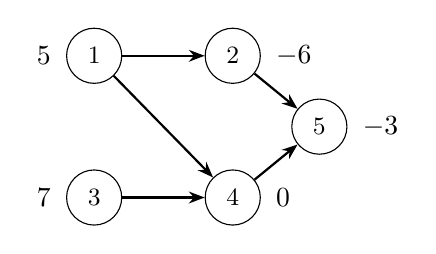
\begin{tikzpicture}[x=1.1cm,y=0.9cm]
  \node[flow node] (n1) at (0,1) {1};
  \node[flow node] (n2) at (1.6,1) {2};
  \node[flow node] (n3) at (0,-1) {3};
  \node[flow node] (n4) at (1.6,-1) {4};
  \node[flow node] (n5) at (2.6,0) {5};
  \node[left=2pt of n1] {\(5\)};
  \node[right=2pt of n2] {\(-6\)};
  \node[left=2pt of n3] {\(7\)};
  \node[right=2pt of n4] {\(0\)};
  \node[right=2pt of n5] {\(-3\)};
  \draw[flow edge] (n1) -- (n2);
  \draw[flow edge] (n1) -- (n4);
  \draw[flow edge] (n2) -- (n5);
  \draw[flow edge] (n3) -- (n4);
  \draw[flow edge] (n4) -- (n5);
\end{tikzpicture}
\caption{Ví dụ đồ thị đóng trọng số: chọn 1 kéo theo 2 và 4, chọn 4 kéo theo 5.}
\end{figure}

Trong thực tế, đồ thị phụ thuộc thường là DAG: muốn chọn một sự kiện thì phải
chọn mọi tiền đề của nó. Ví dụ, kế hoạch học phần ở đại học có các môn học
tiên quyết; nếu mỗi môn có điểm lợi ích, đồ thị đóng trọng số lớn nhất cho
ta kế hoạch có lợi nhất. Với đồ thị có chu trình, mô hình vẫn dùng được, chẳng
hạn trong phân kỳ dự án khi một số hạng mục phụ thuộc lẫn nhau và phải thực
hiện cùng đợt.

\subsection{Cách dựng}

Từ đồ thị \(G=(V,E)\), dựng mạng \(N=(V_N,E_N)\):
\[
\begin{aligned}
V_N &= V\cup\{s,t\},\\
E_N &= E
 \cup\{(s,v)\mid v\in V,\ w_v>0\}
 \cup\{(v,t)\mid v\in V,\ w_v<0\}.
\end{aligned}
\]
Sức chứa:
\[
  c(u,v)=
  \begin{cases}
    \INF, & (u,v)\in E,\\
    w_v, & u=s,\ w_v>0,\\
    -w_v, & v=t,\ w_u<0.
  \end{cases}
\]
Ở đây \(\INF\) là số lớn hơn tổng các trọng số dương, đủ để không thể xuất
hiện trong cắt nhỏ nhất.

\begin{figure}[htbp]
\centering
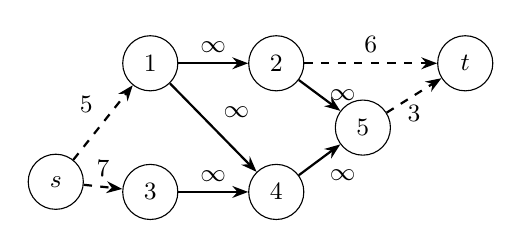
\begin{tikzpicture}[x=1cm,y=0.86cm, every node/.style={font=\small}]
  \node[flow node] (s) at (-1.2,-1) {\(s\)};
  \node[flow node] (n1) at (0,0.75) {1};
  \node[flow node] (n2) at (1.6,0.75) {2};
  \node[flow node] (n3) at (0,-1.15) {3};
  \node[flow node] (n4) at (1.6,-1.15) {4};
  \node[flow node] (n5) at (2.7,-0.2) {5};
  \node[flow node] (t) at (4.0,0.75) {\(t\)};
  \draw[flow weak] (s) -- node[above left]{5} (n1);
  \draw[flow weak] (s) -- node[above]{7} (n3);
  \draw[flow edge] (n1) -- node[above]{\(\infty\)} (n2);
  \draw[flow edge] (n1) -- node[above right]{\(\infty\)} (n4);
  \draw[flow edge] (n2) -- node[right]{\(\infty\)} (n5);
  \draw[flow edge] (n3) -- node[above]{\(\infty\)} (n4);
  \draw[flow edge] (n4) -- node[below right]{\(\infty\)} (n5);
  \draw[flow weak] (n2) -- node[above]{6} (t);
  \draw[flow weak] (n5) -- node[below]{3} (t);
\end{tikzpicture}
\caption{Mạng cắt nhỏ nhất thu được từ đồ thị đóng ở hình trước.}
\end{figure}

\subsection{Chứng minh}

Gọi một cắt \(s\)-\(t\) là \term{cắt đơn} nếu mọi cạnh trong cắt đều kề với
nguồn hoặc đích; nói cách khác, nó không chứa cạnh gốc của \(G\).

\paragraph{Bổ đề 3.1.}
Trong mạng \(N\) ở trên, cắt nhỏ nhất là cắt đơn.

\emph{Chứng minh.}
Các cạnh gốc của \(G\) có sức chứa \(\INF\), còn tổng sức chứa của mọi cạnh
kề nguồn hoặc đích là hữu hạn. Do đó luôn có một cắt hữu hạn, và cắt nhỏ nhất
không thể chứa cạnh sức chứa \(\INF\).

Đặt \(V^+=\{v\mid w_v>0\}\), \(V^-=\{v\mid w_v<0\}\). Với một cắt đơn
\([S,T]\), đặt \(V_1=S-\{s\}\) và \(V_2=V-V_1\).

\paragraph{Bổ đề 3.2 (tính khả thi).}
Các cắt đơn của \(N\) tương ứng một-một với các đồ thị đóng của \(G\) qua
\[
  V_1\cup\{s\}=S.
\]

\emph{Chứng minh.}
Nếu \(V_1\) là đồ thị đóng, cắt \([V_1\cup\{s\}, V_2\cup\{t\}]\) không chứa
cạnh gốc nào: nếu có cạnh \(u\to v\) từ \(V_1\) sang \(V_2\) thì \(V_1\)
không đóng. Ngược lại, nếu cắt là cắt đơn, không có cạnh gốc từ \(V_1\) sang
\(V_2\), nên mọi hậu duệ trực tiếp của đỉnh trong \(V_1\) vẫn nằm trong
\(V_1\); do đó \(V_1\) là đồ thị đóng.

\paragraph{Hệ quả 3.3.}
Trong tương ứng trên,
\[
  c[S,T]=\sum_{v\in V_2^+} w_v+\sum_{v\in V_1^-}(-w_v). \tag{3.1}
\]
Quả vậy, cắt chỉ gồm các cạnh \(s\to V_2^+\) và \(V_1^-\to t\).

\paragraph{Định lý 3.4 (tối ưu).}
Cắt nhỏ nhất của \(N\) tương ứng với đồ thị đóng trọng số lớn nhất của \(G\).

\emph{Chứng minh.}
Trọng số của \(V_1\) là
\[
  w(V_1)=\sum_{v\in V_1^+} w_v-\sum_{v\in V_1^-}(-w_v). \tag{3.2}
\]
Cộng (3.1) và (3.2):
\[
  w(V_1)+c[S,T]
  =\sum_{v\in V_1^+}w_v+\sum_{v\in V_2^+}w_v
  =\sum_{v\in V^+}w_v.
\]
Do đó
\[
  w(V_1)=\sum_{v\in V^+}w_v-c[S,T]. \tag{3.3}
\]
Tổng trọng số dương là hằng số, nên tối thiểu hóa cắt đơn tương đương tối đa
hóa trọng số đồ thị đóng. Theo Bổ đề 3.1, cắt nhỏ nhất là cắt đơn.

Độ phức tạp là \(\Oh(\operatorname{MaxFlow}(N))\).

\subsection{Ứng dụng: Profit}

\paragraph{Mô tả.}
Công ty ADN có \(n\) địa điểm có thể xây trạm trung chuyển. Xây trạm \(i\) tốn
chi phí \(p_i\). Có \(m\) nhóm khách hàng; nhóm \(i\) chỉ được phục vụ nếu
hai trạm \(a_i\) và \(b_i\) đều được xây, và khi đó công ty thu lợi \(c_i\).
Cần chọn các trạm để tối đa hóa
\[
  \text{lợi nhuận ròng}=\text{tổng thu}-\text{tổng chi}.
\]

\paragraph{Lời giải.}
Mỗi nhóm khách hàng là một đỉnh có trọng số dương \(c_i\). Mỗi trạm là một
đỉnh có trọng số âm \(-p_i\). Từ nhóm khách hàng \(i\), nối cạnh có hướng tới
hai trạm \(a_i\) và \(b_i\). Nếu chọn nhóm khách hàng thì bắt buộc chọn hai
trạm, đúng bằng điều kiện đóng. Vì vậy bài toán là một trường hợp của đồ thị
đóng trọng số lớn nhất, giải được trong
\[
  \Oh(\operatorname{MaxFlow}(n+m,n+m)).
\]
Ở phần 4.7, bài viết sẽ chỉ ra một cách nhìn khác đưa bài này về mạng chỉ có
\(n\) đỉnh chính và \(n+m\) cạnh, đạt
\(\Oh(\operatorname{MaxFlow}(n,n+m))\).

\section{Đồ thị con mật độ lớn nhất}

\subsection{Dẫn nhập}

Mật độ của đồ thị vô hướng \(G=(V,E)\) là
\[
  D=\frac{|E|}{|V|}.
\]
Đồ thị con \(G'=(V',E')\) có mật độ lớn nhất là đồ thị con tối đa hóa
\[
  D'=\frac{|E'|}{|V'|}.
\]
Ký hiệu \(n=|V|\), \(m=|E|\). Ví dụ trong một đồ thị sáu đỉnh, nếu bốn đỉnh
bên trong một vùng có năm cạnh nội bộ, mật độ của đồ thị con đó là \(5/4\).

\begin{figure}[htbp]
\centering
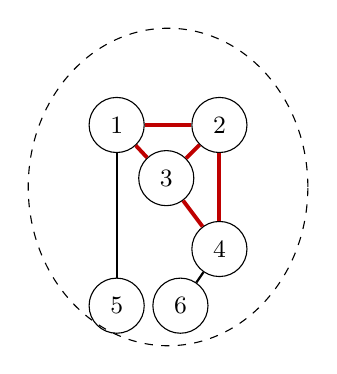
\begin{tikzpicture}[x=0.9cm,y=0.9cm]
  \node[flow node] (n1) at (0,1) {1};
  \node[flow node] (n2) at (1.45,1) {2};
  \node[flow node] (n3) at (0.7,0.25) {3};
  \node[flow node] (n4) at (1.45,-0.75) {4};
  \node[flow node] (n5) at (0,-1.55) {5};
  \node[flow node] (n6) at (0.9,-1.55) {6};
  \node[draw,dashed,ellipse,fit=(n1)(n2)(n3)(n4),inner xsep=7pt,inner ysep=8pt] {};
  \draw[chosen edge] (n1) -- (n2);
  \draw[chosen edge] (n1) -- (n3);
  \draw[chosen edge] (n2) -- (n3);
  \draw[chosen edge] (n2) -- (n4);
  \draw[chosen edge] (n3) -- (n4);
  \draw[thick] (n1) -- (n5);
  \draw[thick] (n4) -- (n6);
\end{tikzpicture}
\caption{Ví dụ đồ thị con mật độ lớn nhất: bốn đỉnh trong nét đứt có năm cạnh,
mật độ \(5/4\).}
\end{figure}

\subsection{Thuật toán chính}

Viết lại bài toán dưới dạng phân thức:
\[
  \max D=f(x)=\frac{\sum_{e\in E}x_e}{\sum_{v\in V}x_v},
\]
trong đó \(x_v,x_e\in\{0,1\}\), và nếu \(e=(u,v)\) được chọn thì \(u,v\) cũng
được chọn.

Với giá trị đoán \(g\), xét
\[
  h(g)=\max_x\left\{\sum_{e\in E}x_e-\sum_{v\in V}g x_v\right\}.
\]
Nếu \(D^*\) là mật độ tối ưu thì
\[
  h(g)=0\Leftrightarrow g=D^*,\qquad
  h(g)<0\Leftrightarrow g>D^*,\qquad
  h(g)>0\Leftrightarrow g<D^*.
\]
Vì vậy có thể nhị phân trên \(g\). Cần xác định số lần nhị phân. Mật độ nằm
giữa \(1/n\) và \(m\).

\paragraph{Bổ đề 4.1.}
Với hai đồ thị con có mật độ khác nhau trong một đồ thị \(n\) đỉnh, hiệu hai
mật độ ít nhất là \(1/n^2\).

\emph{Chứng minh.}
Giả sử \(m_1/n_1>m_2/n_2\). Khi đó
\[
  \frac{m_1}{n_1}-\frac{m_2}{n_2}
  =\frac{m_1n_2-m_2n_1}{n_1n_2}
  \ge \frac1{n_1n_2}\ge \frac1{n^2}.
\]

\paragraph{Hệ quả 4.2.}
Nếu đã có một đồ thị con mật độ \(D\) và không tồn tại đồ thị con nào có mật
độ vượt \(D+1/n^2\), thì nó là đồ thị con mật độ lớn nhất. Do đó số lần nhị
phân cần thiết là \(\Oh(\log n)\), và tổng độ phức tạp là
\[
  \Oh(\log n\cdot \operatorname{Solve}(h(g))).
\]

\subsection{Thuật toán sơ bộ}

Với \(g\) cố định, cần chọn \(G'=(V',E')\) để tối đa hóa
\[
  |E'|-g|V'|.
\]
Ràng buộc là nếu cạnh \(e=(u,v)\) được chọn thì \(u,v\) phải được chọn. Đây
là dạng phụ thuộc của đồ thị đóng. Biến mỗi cạnh \(e\) thành một đỉnh \(v_e\)
có trọng số \(1\); giữ mỗi đỉnh gốc \(v\) với trọng số \(-g\); với mỗi cạnh
\(e=(u,v)\), thêm hai cung \(v_e\to u\) và \(v_e\to v\). Cụ thể:
\[
\begin{aligned}
V_D&=V\cup\{v_e\mid e\in E\},\\
E_D&=\{(v_e,u),(v_e,v)\mid e=(u,v)\in E\},\\
w_{v_e}&=1,\qquad w_v=-g.
\end{aligned}
\]
Bài toán \(h(g)\) trở thành đồ thị đóng trọng số lớn nhất, giải bằng phần 3.
Độ phức tạp là
\[
  \Oh(\log n\cdot \operatorname{MaxFlow}(n+m,n+m)).
\]

\begin{figure}[htbp]
\centering
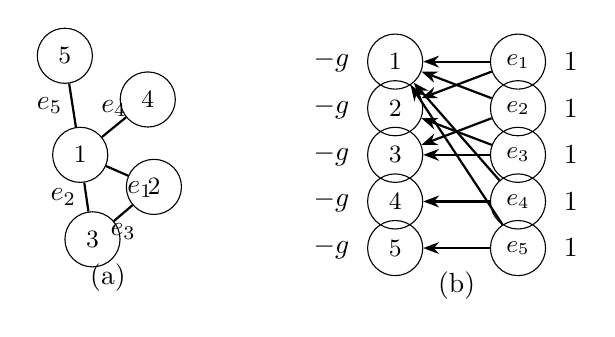
\begin{tikzpicture}[x=0.78cm,y=0.74cm]
  \begin{scope}
    \node[flow node] (a1) at (0,0) {1};
    \node[flow node] (a2) at (1.2,-0.55) {2};
    \node[flow node] (a3) at (0.2,-1.45) {3};
    \node[flow node] (a4) at (1.1,0.95) {4};
    \node[flow node] (a5) at (-0.25,1.7) {5};
    \draw[thick] (a1)--node[below right]{\(e_1\)}(a2);
    \draw[thick] (a1)--node[left]{\(e_2\)}(a3);
    \draw[thick] (a2)--node[below]{\(e_3\)}(a3);
    \draw[thick] (a1)--node[above]{\(e_4\)}(a4);
    \draw[thick] (a1)--node[left]{\(e_5\)}(a5);
    \node at (0.45,-2.1) {(a)};
  \end{scope}
  \begin{scope}[xshift=4.0cm]
    \foreach \i/\y in {1/1.6,2/0.8,3/0,4/-0.8,5/-1.6}{
      \node[flow node] (v\i) at (0,\y) {\i};
      \node[left=0.1cm of v\i] {\(-g\)};
      \node[flow node] (e\i) at (2.0,\y) {\(e_{\i}\)};
      \node[right=0.1cm of e\i] {1};
    }
    \draw[flow edge] (e1)--(v1); \draw[flow edge] (e1)--(v2);
    \draw[flow edge] (e2)--(v1); \draw[flow edge] (e2)--(v3);
    \draw[flow edge] (e3)--(v2); \draw[flow edge] (e3)--(v3);
    \draw[flow edge] (e4)--(v1); \draw[flow edge] (e4)--(v4);
    \draw[flow edge] (e5)--(v1); \draw[flow edge] (e5)--(v5);
    \node at (1,-2.25) {(b)};
  \end{scope}
\end{tikzpicture}
\caption{Thuật toán sơ bộ cho đồ thị con mật độ lớn nhất: mỗi cạnh của \(G\)
trở thành một đỉnh trọng số 1 trong đồ thị đóng.}
\end{figure}

\subsection{Thuật toán cải tiến}

Thuật toán sơ bộ biến cạnh thành đỉnh, làm mô hình tổng quát hơn mức cần
thiết. Ta khai thác tính chất riêng của đồ thị con mật độ.

Với tập đỉnh \(V'\) cố định, để tối đa hóa \(|E'|-g|V'|\), rõ ràng nên chọn
tất cả cạnh trong đồ thị con cảm sinh bởi \(V'\). Vì vậy \(E'\) có thể được
định nghĩa lại là tập mọi cạnh có hai đầu đều thuộc \(V'\).

Thay vì chọn trực tiếp các cạnh trong \(E'\), nhìn vào các cạnh đi giữa
\(V'\) và phần bù \(\overline{V'}\). Với \(d_v\) là bậc của \(v\),

\begin{figure}[htbp]
\centering
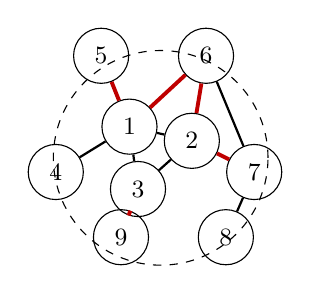
\begin{tikzpicture}[x=0.72cm,y=0.72cm]
  \node[flow node] (n1) at (0,0) {1};
  \node[flow node] (n2) at (1.1,-0.25) {2};
  \node[flow node] (n3) at (0.15,-1.1) {3};
  \node[flow node] (n4) at (-1.3,-0.8) {4};
  \node[flow node] (n5) at (-0.5,1.25) {5};
  \node[flow node] (n6) at (1.35,1.25) {6};
  \node[flow node] (n7) at (2.2,-0.8) {7};
  \node[flow node] (n8) at (1.7,-1.95) {8};
  \node[flow node] (n9) at (-0.15,-1.95) {9};
  \node[draw,dashed,ellipse,fit=(n1)(n2)(n3),inner sep=6pt] {};
  \draw[thick] (n1)--(n2)--(n3)--(n1);
  \draw[chosen edge] (n5)--(n1);
  \draw[chosen edge] (n6)--(n1);
  \draw[chosen edge] (n6)--(n2);
  \draw[chosen edge] (n7)--(n2);
  \draw[chosen edge] (n9)--(n3);
  \draw[thick] (n4)--(n1);
  \draw[thick] (n6)--(n7)--(n8);
\end{tikzpicture}
\caption{Tư duy bổ sung trong thuật toán cải tiến: thay vì chọn cạnh nội bộ,
xét các cạnh đỏ đi giữa \(V'\) và \(\overline{V'}\).}
\end{figure}

\[
\begin{aligned}
\min\; g|V'|-|E'|
&=\sum_{v\in V'}g-
  \left(\frac{\sum_{v\in V'}d_v-c[V',\overline{V'}]}2\right)\\
&=\sum_{v\in V'}\left(g-\frac{d_v}{2}\right)
  +\frac12c[V',\overline{V'}].
\end{aligned}
\]
Nhân đôi mục tiêu:
\[
  \sum_{v\in V'}(2g-d_v)+2c[V',\overline{V'}].
\]

Dựng mạng \(N=(V_N,E_N)\) như sau:
\[
\begin{aligned}
V_N&=V\cup\{s,t\},\\
E_N&=\{(u,v),(v,u)\mid (u,v)\in E\}
\cup\{(s,v),(v,t)\mid v\in V\}.
\end{aligned}
\]
Sức chứa:
\[
  c(u,v)=1\quad((u,v)\in E),\qquad
  c(s,v)=U,\qquad
  c(v,t)=U+2g-d_v.
\]
Vì \(d_v\le m\) và \(g\ge 0\), chọn \(U=m\) đủ để mọi sức chứa không âm.

\begin{figure}[htbp]
\centering
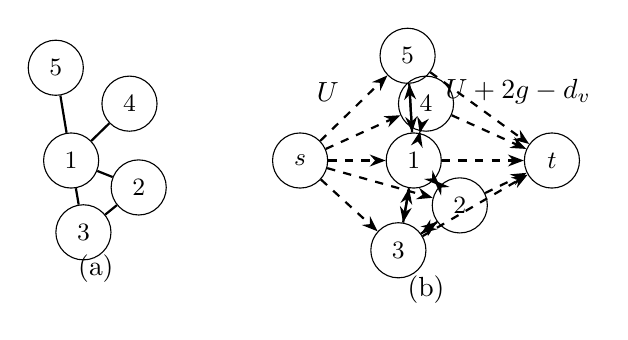
\begin{tikzpicture}[x=0.78cm,y=0.76cm]
  \begin{scope}
    \node[flow node] (a1) at (0,0) {1};
    \node[flow node] (a2) at (1.1,-0.45) {2};
    \node[flow node] (a3) at (0.2,-1.2) {3};
    \node[flow node] (a4) at (0.95,0.95) {4};
    \node[flow node] (a5) at (-0.25,1.55) {5};
    \draw[thick] (a1)--(a2)--(a3)--(a1)--(a4);
    \draw[thick] (a1)--(a5);
    \node at (0.4,-1.8) {(a)};
  \end{scope}
  \begin{scope}[xshift=4.0cm]
    \node[flow node] (s) at (-1.4,0) {\(s\)};
    \node[flow node] (t) at (2.7,0) {\(t\)};
    \node[flow node] (n1) at (0.45,0) {1};
    \node[flow node] (n2) at (1.2,-0.75) {2};
    \node[flow node] (n3) at (0.2,-1.5) {3};
    \node[flow node] (n4) at (0.65,0.95) {4};
    \node[flow node] (n5) at (0.35,1.75) {5};
    \foreach \u/\v in {n1/n2,n2/n3,n3/n1,n1/n4,n1/n5}{
      \draw[flow edge] (\u) -- (\v);
      \draw[flow edge] (\v) -- (\u);
    }
    \foreach \v in {n1,n2,n3,n4,n5}{
      \draw[flow weak] (s) -- (\v);
      \draw[flow weak] (\v) -- (t);
    }
    \node at (-0.95,1.15) {\(U\)};
    \node at (2.15,1.15) {\(U+2g-d_v\)};
    \node at (0.65,-2.15) {(b)};
  \end{scope}
\end{tikzpicture}
\caption{Cách dựng mạng của thuật toán cải tiến: cạnh gốc có sức chứa 1 theo
hai hướng, còn trọng số đỉnh được chuyển sang các cạnh kề nguồn và đích.}
\end{figure}

\subsection{Chứng minh thuật toán cải tiến}

\paragraph{Bổ đề 4.3.}
Với \(V'\) cố định, chọn \(E'\) là tập cạnh của đồ thị con cảm sinh bởi \(V'\)
là phương án tối ưu cho \(h(g)\).

\paragraph{Bổ đề 4.4 (tính khả thi).}
Mỗi cắt \([S,T]\) của mạng \(N\) tương ứng một-một với một tập đỉnh
\(V'=S-\{s\}\) của đồ thị gốc.

\paragraph{Định lý 4.5 (tối ưu).}
Cắt nhỏ nhất của \(N\) cho nghiệm tối ưu của \(h(g)\).

\emph{Chứng minh.}
Với \(V'=S-\{s\}\), \(\overline{V'}=T-\{t\}\),
\[
\begin{aligned}
c[S,T]
&=\sum_{v\in\overline{V'}} c(s,v)
  +\sum_{u\in V'} c(u,t)
  +\sum_{\substack{u\in V',\,v\in\overline{V'}\\(u,v)\in E}} c(u,v)\\
&=\sum_{v\in\overline{V'}} U
  +\sum_{u\in V'}(U+2g-d_u)
  +\sum_{\substack{u\in V',\,v\in\overline{V'}\\(u,v)\in E}}1\\
&=Un+\sum_{u\in V'}
  \left(2g-d_u+\sum_{\substack{v\in\overline{V'}\\(u,v)\in E}}1\right)\\
&=Un+\sum_{u\in V'}
  \left(2g-\sum_{\substack{v\in V'\\(u,v)\in E}}1\right)\\
&=Un+2g|V'|-2|E'|\\
&=Un-2(|E'|-g|V'|).
\end{aligned}
\]
Do \(Un\) là hằng số, cắt càng nhỏ thì \(|E'|-g|V'|\) càng lớn. Hơn nữa
\[
  h(g)=\frac{Un-c[S,T]}2
\]
khi \([S,T]\) là cắt nhỏ nhất.

Vì mạng có \(n+2\) đỉnh và \(\Theta(n+m)\) cạnh, độ phức tạp toàn bộ là
\[
  \Oh(\log n\cdot \operatorname{MaxFlow}(n,n+m)).
\]

\subsection{Mở rộng tới đồ thị có trọng số cạnh}

Cho đồ thị vô hướng \(G=(V,E)\), mỗi cạnh có trọng số không âm \(w_e\). Mật độ
được định nghĩa là
\[
  D=\frac{\sum_{e\in E}w_e}{|V|}.
\]
Với \(g\) cố định, cần tối đa hóa
\[
  \sum_{e\in E'}w_e-g|V'|. \tag{4.2}
\]
Thuật toán cải tiến vẫn dùng được nếu định nghĩa
\[
  d_u=\sum_{(u,v)\in E} w_{(u,v)}.
\]
Trong mạng, sức chứa hai cung thay cho cạnh \((u,v)\) là \(w_{(u,v)}\), chọn
\[
  U=\sum_{e\in E} w_e,
\]
và giữ \(c(v,t)=U+2g-d_v\). Khi đó vẫn có
\[
  h(g)=\frac{Un-c[S,T]}2.
\]
Do mật độ có trọng số không còn đảm bảo khoảng cách \(1/n^2\), số lần nhị
phân phụ thuộc độ chính xác đặt trước. Nếu số lần nhị phân là \(k\), độ phức
tạp là
\[
  \Oh(k\cdot \operatorname{MaxFlow}(n,n+m)).
\]

\subsection{Mở rộng tới đồ thị có trọng số đỉnh và cạnh}

Cho đồ thị vô hướng \(G=(V,E)\), mỗi đỉnh có trọng số \(p_v\in\R\), mỗi cạnh
có trọng số không âm \(w_e\). Mật độ được định nghĩa là
\[
  D=\frac{\sum_{v\in V}p_v+\sum_{e\in E}w_e}{|V|}.
\]
Với \(g\) cố định, bài toán con là tối đa hóa
\[
  \sum_{e\in E'}w_e+\sum_{v\in V'}p_v-\sum_{v\in V'}g
  =\sum_{e\in E'}w_e-\sum_{v\in V'}(g-p_v). \tag{4.3}
\]
So với phần trước, chỉ cần thay \(g\) bởi \(g-p_v\) tại đỉnh \(v\). Đặt
\[
  d_u=\sum_{(u,v)\in E} w_{(u,v)},\qquad
  U=2\sum_{v\in V}|p_v|+\sum_{e\in E}w_e.
\]
Dựng mạng:
\[
\begin{aligned}
V_N&=V\cup\{s,t\},\\
E_N&=\{(u,v),(v,u)\mid (u,v)\in E\}
\cup\{(s,v),(v,t)\mid v\in V\},
\end{aligned}
\]
với
\[
  c(u,v)=w_{(u,v)},\qquad
  c(s,v)=U,\qquad
  c(v,t)=U+2g-d_v-2p_v.
\]
Khi đó \(h(g)=(Un-c[S,T])/2\) với cắt nhỏ nhất. Độ phức tạp là
\[
  \Oh(k\cdot \operatorname{MaxFlow}(n,n+m)).
\]

\subsection{Ứng dụng}

\subsubsection{Hard Life}

\paragraph{Mô tả.}
Công ty ADN có \(n\) nhân viên. Giữa một số cặp nhân viên có mâu thuẫn; mỗi
mâu thuẫn là một cạnh. Cần chọn danh sách sa thải sao cho ``tỷ lệ bất hòa''
của nhóm bị sa thải là lớn nhất:
\[
  \frac{\text{số mâu thuẫn nội bộ trong nhóm}}{\text{số nhân viên trong nhóm}}.
\]

\paragraph{Lời giải.}
Đây chính là bài toán đồ thị con mật độ lớn nhất. Dùng trực tiếp thuật toán
trong phần này.

\subsubsection{Profit}

\paragraph{Mô tả.}
Giống phần 3.4.

\paragraph{Lời giải.}
Xem nhóm khách hàng là cạnh, trạm trung chuyển là đỉnh. Chọn một cạnh nghĩa là
phục vụ nhóm khách hàng và nhận lợi ích \(w_e\); chọn một đỉnh nghĩa là xây
trạm và trả chi phí \(p_v\). Mục tiêu là
\[
  \max \sum_{e\in E'}w_e-\sum_{v\in V'}p_v.
\]
Ràng buộc: nếu chọn cạnh \(e=(u,v)\) thì phải chọn cả hai đầu \(u,v\). Đây
cũng là ràng buộc của mô hình đồ thị con mật độ có trọng số đỉnh và cạnh.
Trong công thức (4.3), nếu lấy \(g-p_v\) đúng bằng chi phí \(p_v\) của bài
Profit, ta thu được mục tiêu trên. Vì không cần nhị phân theo mật độ, bài này
giải trực tiếp bằng một lần cắt nhỏ nhất trên mạng kích thước \(n\) đỉnh chính
và \(n+m\) cạnh:
\[
  \Oh(\operatorname{MaxFlow}(n,n+m)).
\]
So với cách đồ thị đóng \(\Oh(\operatorname{MaxFlow}(n+m,n+m))\), đây là cải
tiến bản chất và đạt tới quy mô cùng bậc với dữ liệu đầu vào.

\section{Tập phủ đỉnh và tập độc lập trong đồ thị hai phía}

\subsection{Dẫn nhập}

Trong đồ thị vô hướng \(G=(V,E)\), \term{tập phủ đỉnh} là tập \(V'\subseteq V\)
sao cho mọi cạnh có ít nhất một đầu mút thuộc \(V'\):
\[
  \forall (u,v)\in E,\quad u\in V'\ \text{hoặc}\ v\in V'.
\]
\term{Tập độc lập đỉnh} là tập \(V'\subseteq V\) sao cho không có hai đỉnh nào
trong tập kề nhau; tương đương, với mọi cạnh \((u,v)\), không thể đồng thời
có \(u,v\in V'\).

Tập phủ đỉnh nhỏ nhất và tập độc lập đỉnh lớn nhất là các bài toán kinh điển
khó trong đồ thị tổng quát, nhưng trên đồ thị hai phía có thể giải nhanh nhờ
matching. Phần này xét bản mở rộng có trọng số đỉnh không âm: tìm tập phủ có
tổng trọng số nhỏ nhất và tập độc lập có tổng trọng số lớn nhất trong đồ thị
hai phía \(G=(X\cup Y,E)\).

\subsection{Tập phủ đỉnh trọng số nhỏ nhất}

Với đồ thị hai phía \(G=(X\cup Y,E)\), dựng mạng \(N=(V_N,E_N)\):
\[
\begin{aligned}
V_N&=V\cup\{s,t\},\\
E_N&=E\cup\{(s,u)\mid u\in X\}\cup\{(v,t)\mid v\in Y\}.
\end{aligned}
\]
Hướng các cạnh của \(E\) từ \(X\) sang \(Y\). Sức chứa:
\[
  c(u,v)=\INF\quad((u,v)\in E),\qquad
  c(s,u)=w_u\quad(u\in X),\qquad
  c(v,t)=w_v\quad(v\in Y).
\]

\begin{figure}[htbp]
\centering
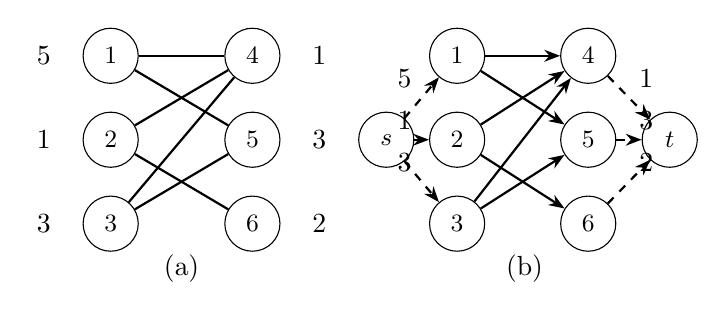
\begin{tikzpicture}[x=0.9cm,y=0.82cm]
  \begin{scope}
    \foreach \i/\y/\w in {1/1.3/5,2/0/1,3/-1.3/3}{
      \node[flow node] (x\i) at (0,\y) {\i};
      \node[left=0.28cm of x\i] {\w};
    }
    \foreach \i/\y/\w in {4/1.3/1,5/0/3,6/-1.3/2}{
      \node[flow node] (y\i) at (2.0,\y) {\i};
      \node[right=0.28cm of y\i] {\w};
    }
    \draw[thick] (x1)--(y4);
    \draw[thick] (x1)--(y5);
    \draw[thick] (x2)--(y4);
    \draw[thick] (x2)--(y6);
    \draw[thick] (x3)--(y4);
    \draw[thick] (x3)--(y5);
    \node at (1,-2.0) {(a)};
  \end{scope}
  \begin{scope}[xshift=4.4cm]
    \node[flow node] (s) at (-1.0,0) {\(s\)};
    \node[flow node] (t) at (3.0,0) {\(t\)};
    \foreach \i/\y/\w in {1/1.3/5,2/0/1,3/-1.3/3}{
      \node[flow node] (x\i) at (0,\y) {\i};
      \draw[flow weak] (s) -- node[above left]{\w} (x\i);
    }
    \foreach \i/\y/\w in {4/1.3/1,5/0/3,6/-1.3/2}{
      \node[flow node] (y\i) at (1.85,\y) {\i};
      \draw[flow weak] (y\i) -- node[above right]{\w} (t);
    }
    \draw[flow edge] (x1)--(y4);
    \draw[flow edge] (x1)--(y5);
    \draw[flow edge] (x2)--(y4);
    \draw[flow edge] (x2)--(y6);
    \draw[flow edge] (x3)--(y4);
    \draw[flow edge] (x3)--(y5);
    \node at (0.95,-2.0) {(b)};
  \end{scope}
\end{tikzpicture}
\caption{Chuyển đồ thị hai phía có trọng số đỉnh thành mạng cắt nhỏ nhất cho
bài tập phủ đỉnh trọng số nhỏ nhất.}
\end{figure}

Mọi đường từ \(s\) tới \(t\) có dạng \(s\to u\to v\to t\). Một cắt phải chặn
mỗi đường như vậy. Vì cạnh \(u\to v\) có sức chứa \(\INF\), cắt nhỏ nhất sẽ
chọn ít nhất một trong hai cạnh \(s\to u\) hoặc \(v\to t\), đúng với điều kiện
``ít nhất một đầu mút của mỗi cạnh được phủ''.

\paragraph{Bổ đề 5.1.}
Cắt đơn của \(N\) tương ứng một-một với tập phủ đỉnh \(V'=X'\cup Y'\):
\[
  [S,T]=[\{s\},X']\cup[Y',\{t\}].
\]
Sức chứa cắt đúng bằng tổng trọng số các đỉnh được chọn. Do đó cắt nhỏ nhất
cho tập phủ đỉnh trọng số nhỏ nhất, với độ phức tạp
\[
  \Oh(\operatorname{MaxFlow}(N)).
\]

\subsection{Tập độc lập đỉnh trọng số lớn nhất}

Điều kiện độc lập là
\[
  \neg(u\in V'\ \text{và}\ v\in V')
  \quad\Leftrightarrow\quad
  u\notin V'\ \text{hoặc}\ v\notin V'.
\]
Vế phải giống điều kiện phủ nếu xét phần bù.

\paragraph{Định lý 5.2 (phủ và độc lập bù nhau).}
Trong một đồ thị không xét các đỉnh cô lập, \(V'\) là tập phủ đỉnh khi và chỉ
khi \(V-V'\) là tập độc lập.

\emph{Chứng minh.}
Nếu \(V'\) là tập phủ mà \(V-V'\) chứa hai đỉnh kề \(u,v\), cạnh \((u,v)\)
không được phủ, mâu thuẫn. Ngược lại, nếu \(V-V'\) là độc lập mà tồn tại cạnh
\((u,v)\) không được phủ bởi \(V'\), thì \(u,v\in V-V'\), mâu thuẫn.

\begin{figure}[htbp]
\centering
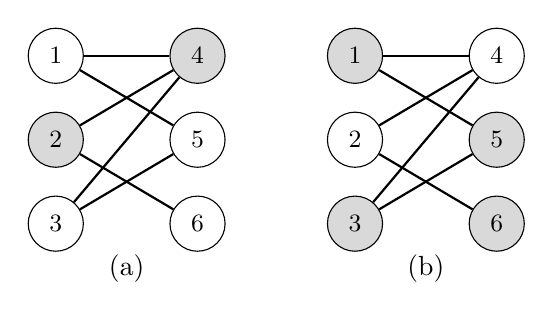
\begin{tikzpicture}[x=0.9cm,y=0.82cm]
  \begin{scope}
    \node[flow node] (x1) at (0,1.3) {1};
    \node[flow node,fill=gray!30] (x2) at (0,0) {2};
    \node[flow node] (x3) at (0,-1.3) {3};
    \node[flow node,fill=gray!30] (y4) at (2.0,1.3) {4};
    \node[flow node] (y5) at (2.0,0) {5};
    \node[flow node] (y6) at (2.0,-1.3) {6};
    \draw[thick] (x1)--(y4);
    \draw[thick] (x1)--(y5);
    \draw[thick] (x2)--(y4);
    \draw[thick] (x2)--(y6);
    \draw[thick] (x3)--(y4);
    \draw[thick] (x3)--(y5);
    \node at (1,-2.0) {(a)};
  \end{scope}
  \begin{scope}[xshift=3.8cm]
    \node[flow node,fill=gray!30] (x1) at (0,1.3) {1};
    \node[flow node] (x2) at (0,0) {2};
    \node[flow node,fill=gray!30] (x3) at (0,-1.3) {3};
    \node[flow node] (y4) at (2.0,1.3) {4};
    \node[flow node,fill=gray!30] (y5) at (2.0,0) {5};
    \node[flow node,fill=gray!30] (y6) at (2.0,-1.3) {6};
    \draw[thick] (x1)--(y4);
    \draw[thick] (x1)--(y5);
    \draw[thick] (x2)--(y4);
    \draw[thick] (x2)--(y6);
    \draw[thick] (x3)--(y4);
    \draw[thick] (x3)--(y5);
    \node at (1,-2.0) {(b)};
  \end{scope}
\end{tikzpicture}
\caption{Tập phủ đỉnh và tập độc lập bù nhau: các đỉnh tô xám trong (a) là
một tập phủ, còn các đỉnh tô xám trong (b) là phần bù độc lập của nó.}
\end{figure}

\paragraph{Hệ quả 5.3 (tối ưu).}
Nếu \(V'\) là tập phủ đỉnh trọng số nhỏ nhất thì \(V-V'\) là tập độc lập đỉnh
trọng số lớn nhất. Vì
\[
  \sum_{v\in V}w_v=\sum_{v\in V'}w_v+\sum_{v\in V-V'}w_v
\]
là hằng số, tối thiểu hóa trọng số phần phủ tương đương tối đa hóa trọng số
phần bù độc lập. Độ phức tạp vẫn là \(\Oh(\operatorname{MaxFlow}(N))\).

\subsection{Ứng dụng}

\subsubsection{Destroying the Graph}

\paragraph{Mô tả.}
Cho đồ thị có hướng \(D=(V,E)\). Với mỗi đỉnh \(u\) có hai thao tác:
\begin{itemize}
  \item \(a(u)\): xóa mọi cạnh đi ra từ \(u\), chi phí \(c_a(u)\);
  \item \(b(u)\): xóa mọi cạnh đi vào \(u\), chi phí \(c_b(u)\).
\end{itemize}
Cần xóa toàn bộ cạnh với chi phí nhỏ nhất.

\paragraph{Lời giải.}
Xét một cạnh có hướng \((u,v)\). Nó chỉ có thể bị xóa bởi \(a(u)\) hoặc
\(b(v)\), nên ít nhất một trong hai thao tác phải được chọn. Đây là điều kiện
tập phủ.

Tách mỗi đỉnh \(v\) thành hai đỉnh \(v_a\) và \(v_b\), tương ứng thao tác
\(a(v)\) và \(b(v)\). Với mỗi cạnh \((u,v)\in E\), thêm cạnh hai phía
\(u_a v_b\). Đặt
\[
  X=\{u_a\mid u\in V\},\qquad
  Y=\{v_b\mid v\in V\},
\]
\[
  E_G=\{(u_a,v_b)\mid (u,v)\in E\},\qquad
  w_{u_a}=c_a(u),\quad w_{v_b}=c_b(v).
\]
Đây là đồ thị hai phía. Một tập thao tác xóa hết cạnh tương ứng đúng với một
tập phủ đỉnh trong đồ thị này. Dùng thuật toán phần 5.2.

\subsubsection{Exca}

\paragraph{Mô tả.}
Cho lưới \(n\times m\), mỗi ô có một viên đá quý giá trị \(v_{i,j}\). Amber
tự chọn ô bắt đầu ở giây \(0\). Trong mỗi giây, theo thứ tự:
\begin{enumerate}
  \item nếu đầu giây \(i\) Amber ở \((x,y)\), có thể lấy đá quý tại ô đó;
  \item nếu \(i\) chẵn, đá quý ở bốn ô kề cạnh với \((x,y)\) biến mất;
  \item trước đầu giây \(i+1\), Amber có thể đi sang một ô kề cạnh hoặc đứng
  yên.
\end{enumerate}
Cần tối đa hóa tổng giá trị đá quý lấy được.

\begin{figure}[htbp]
\centering
\begin{tikzpicture}[x=0.58cm,y=0.58cm, every node/.style={font=\scriptsize}]
  \foreach \x/\y/\title/\a/\b/\c/\d in {
    0/2.1/Ban đầu/4/1/2/3,
    -4/-1.0/Giây 0/4/1/2/0,
    -1.5/-1.0/Giây 0/4/0/0/0,
    1/-1.0/Giây 0/4/0/0/0,
    3.5/-1.0/Giây 1/4/0/0/0,
    6/-1.0/Giây 1/4/0/0/0,
    8.5/-1.0/Giây 2/0/0/0/0}{
      \node[above] at (\x+1,\y+0.15) {\title};
      \draw (\x,\y) rectangle ++(1,-1);
      \draw (\x+1,\y) rectangle ++(1,-1);
      \draw (\x,\y-1) rectangle ++(1,-1);
      \draw (\x+1,\y-1) rectangle ++(1,-1);
      \node at (\x+0.5,\y-0.5) {\a};
      \node at (\x+1.5,\y-0.5) {\b};
      \node at (\x+0.5,\y-1.5) {\c};
      \node at (\x+1.5,\y-1.5) {\d};
  }
  \node[left] at (-0.25,1.6) {A};
  \node[left] at (-0.25,1.0) {B};
  \node[above] at (0.5,2.45) {1};
  \node[above] at (1.5,2.45) {2};
  \node[draw,circle,inner sep=1pt] at (-2.5,-2.5) {0};
  \node[draw,circle,inner sep=1pt] at (1.5,-1.5) {0};
  \node[draw,circle,inner sep=1pt] at (1.5,-2.5) {0};
  \node[draw,circle,inner sep=1pt] at (5.0,-1.5) {0};
  \draw[-{Stealth[length=1.5mm]},gray,line width=1pt] (7.5,-1.5) -- (6.5,-1.5);
  \node[draw,circle,inner sep=1pt] at (7.5,-1.5) {0};
  \node[draw,circle,inner sep=1pt] at (9.0,-1.5) {0};
\end{tikzpicture}
\caption{Ví dụ \(2\times 2\) của Exca: lấy B2 ở giây 0, đi qua A2/A1 và lấy
được thêm A1 ở giây 2.}
\end{figure}

\paragraph{Bổ đề 5.5.}
Chỉ có thể lấy đá quý ở các giây chẵn.

\emph{Chứng minh.}
Nếu lấy ngay tại vị trí khởi đầu thì đó là giây \(0\), chẵn. Với một ô \(B\)
được đi vào từ ô kề \(A\), giả sử lấy được đá quý ở giây lẻ. Một giây trước
đó là giây chẵn, Amber ở \(A\), nên đá quý ở các ô kề \(A\), trong đó có
\(B\), đã biến mất. Mâu thuẫn.

\paragraph{Hệ quả 5.6.}
Không thể lấy đá quý ở hai ô kề cạnh nhau. Nếu lấy viên thứ nhất ở giây chẵn,
mọi viên ở ô kề nó biến mất ngay trong giây đó, nên viên kề cạnh không thể
được lấy sau.

Vậy các ô được lấy tạo thành một tập độc lập trên đồ thị lưới, mỗi ô là một
đỉnh và hai ô kề cạnh nối bởi một cạnh. Cần thêm chiều ngược lại: mọi tập độc
lập đều có thể hiện thực bằng một đường đi.

\paragraph{Định lý 5.7.}
Với mọi tập độc lập trên lưới, tồn tại một lịch di chuyển lấy được toàn bộ đá
quý trong tập đó.

\emph{Ý tưởng chứng minh.}
Duyệt lưới theo từng cặp hàng. Trong mỗi giai đoạn gồm hai hàng, đi dọc hàng
thứ nhất theo thứ tự trái sang phải hoặc phải sang trái. Nếu cần lấy đá ở
hàng thứ nhất, đi vào ô đó ở giây chẵn. Nếu cần lấy đá ở hàng thứ hai, đi
vào ô tương ứng ở hàng thứ nhất ở giây lẻ, bước xuống lấy đá ở hàng thứ hai,
rồi quay lại; quá trình này dùng hai giây nên giữ nguyên tính chẵn lẻ cho
đường đi chính.

\begin{figure}[htbp]
\centering
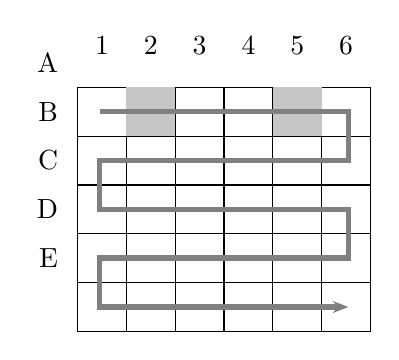
\begin{tikzpicture}[x=0.62cm,y=0.62cm]
  \foreach \r/\name in {0/A,1/B,2/C,3/D,4/E}{
    \node[left] at (-0.2,-\r+0.5) {\name};
  }
  \foreach \c in {1,...,6}{
    \node at (\c-0.5,0.85) {\c};
  }
  \foreach \r in {0,...,4}{
    \foreach \c in {0,...,5}{
      \draw (\c,-\r) rectangle ++(1,-1);
    }
  }
  \fill[gray!45] (1,0) rectangle (2,-1);
  \fill[gray!45] (4,0) rectangle (5,-1);
  \draw[gray,line width=2pt,-{Stealth[length=2mm]}] (0.45,-0.5)--(5.55,-0.5)--(5.55,-1.5)--(0.45,-1.5)--(0.45,-2.5)--(5.55,-2.5)--(5.55,-3.5)--(0.45,-3.5)--(0.45,-4.5)--(5.55,-4.5);
\end{tikzpicture}
\caption{Đường đi chữ Z đơn giản có thể làm sai chẵn lẻ giữa hai hàng, nên
nguồn chuyển sang chứng minh theo từng giai đoạn hai hàng.}
\end{figure}

Các giai đoạn không ảnh hưởng lẫn nhau: giai đoạn trước đã lấy xong; khi giai
đoạn hiện tại bước xuống hàng thứ hai, do tập là độc lập, ô cùng cột ở hàng
kế tiếp của giai đoạn sau không cần lấy. Trong một giai đoạn, mã hóa yêu cầu
trên hàng chính bằng chuỗi \(0,1,?\): \(0\) nghĩa là phải vào ô ở giây chẵn,
\(1\) nghĩa là phải vào ô ở giây lẻ để lấy viên ở hàng phụ, còn \(?\) là tự do.
Vì tập độc lập, các yêu cầu xác định không tạo hai ký hiệu bằng nhau liên tiếp
mà không có khoảng trống phù hợp. Các đoạn \(?\) có thể được gán chẵn lẻ hoặc
thêm một lần đứng yên để khớp hai phía. Do đó luôn dựng được lịch.

\begin{figure}[htbp]
\centering
\begin{tikzpicture}[x=0.62cm,y=0.62cm]
  \foreach \r/\name in {0/A,1/B,2/C,3/D,4/E}{
    \node[left] at (-0.2,-\r+0.5) {\name};
  }
  \foreach \c in {1,...,6}{
    \node at (\c-0.5,0.85) {\c};
  }
  \foreach \r in {0,...,4}{
    \foreach \c in {0,...,5}{
      \draw (\c,-\r) rectangle ++(1,-1);
    }
  }
  \fill[gray!45] (1,0) rectangle (2,-1);
  \fill[gray!45] (2,-1) rectangle (3,-2);
  \fill[gray!45] (4,0) rectangle (5,-1);
  \fill[gray!45] (4,-2) rectangle (5,-3);
  \fill[gray!45] (5,-3) rectangle (6,-4);
  \draw[gray,line width=2pt,-{Stealth[length=2mm]}] (0.45,-0.5)--(2.45,-0.5)--(2.45,-1.5)--(2.45,-0.5)--(5.55,-0.5)--(5.55,-1.5);
  \draw[gray,line width=2pt,-{Stealth[length=2mm]}] (5.55,-2.5)--(0.45,-2.5)--(0.45,-4.5)--(5.55,-4.5);
  \draw[decorate,decoration={brace,amplitude=4pt}] (6.25,0) -- node[right=5pt]{Giai đoạn 1} (6.25,-2);
  \draw[decorate,decoration={brace,amplitude=4pt}] (6.25,-2) -- node[right=5pt]{Giai đoạn 2} (6.25,-4);
\end{tikzpicture}
\caption{Chia thành các giai đoạn hai hàng: đi xuống hàng phụ rồi quay lại
giữ nguyên chẵn lẻ của đường đi chính.}
\end{figure}

\begin{figure}[htbp]
\centering
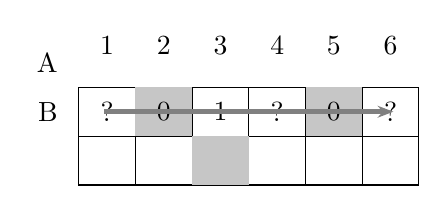
\begin{tikzpicture}[x=0.72cm,y=0.62cm]
  \foreach \r/\name in {0/A,1/B}{
    \node[left] at (-0.2,-\r+0.5) {\name};
  }
  \foreach \c in {1,...,6}{
    \node at (\c-0.5,0.85) {\c};
  }
  \foreach \r in {0,1}{
    \foreach \c in {0,...,5}{
      \draw (\c,-\r) rectangle ++(1,-1);
    }
  }
  \fill[gray!45] (1,0) rectangle (2,-1);
  \fill[gray!45] (2,-1) rectangle (3,-2);
  \fill[gray!45] (4,0) rectangle (5,-1);
  \node at (0.5,-0.5) {?};
  \node at (1.5,-0.5) {0};
  \node at (2.5,-0.5) {1};
  \node at (3.5,-0.5) {?};
  \node at (4.5,-0.5) {0};
  \node at (5.5,-0.5) {?};
  \draw[gray,line width=2pt,-{Stealth[length=2mm]}] (0.45,-0.5)--(5.55,-0.5);
\end{tikzpicture}
\caption{Chuỗi yêu cầu \(0,1,?\) trên một giai đoạn: \(0\) là vào ô ở giây
chẵn, \(1\) là vào ở giây lẻ để lấy viên ở hàng dưới, còn \(?\) có thể gán để
nối hai phía.}
\end{figure}

Vì đồ thị lưới là đồ thị hai phía theo tô màu đen trắng bàn cờ, bài toán Exca
trở thành tập độc lập đỉnh trọng số lớn nhất trong đồ thị hai phía. Dùng phần
5.3 để giải.

\section{Kết luận}

Cắt nhỏ nhất là đối ngẫu của luồng cực đại, nhưng trừu tượng hơn và khó dựng
hơn từ trực giác vật lý. Các ví dụ trong bài chỉ bao phủ vài lớp thường gặp;
điều quan trọng hơn là nắm được cách phân tích.

\subsection{Khuôn mẫu biến đổi}

Mọi bài toán ở trên đều được quy về cắt nhỏ nhất bằng cách xây dựng tương ứng
một-một giữa phương án của bài toán gốc và một lớp cắt có tính chất đặc biệt,
đồng thời chứng minh cắt nhỏ nhất chắc chắn nằm trong lớp đó. Ở phần đồ thị
đóng, cắt đơn tương ứng với tập đóng, và cắt nhỏ nhất luôn là cắt đơn vì các
cạnh phụ thuộc có sức chứa \(\INF\).

\subsection{Tính chất của cắt}

\paragraph{Tính chất 1: ngắt đường.}
Sau khi bỏ các cạnh của một cắt, không còn đường nào từ nguồn tới đích. Trong
bài tập phủ đỉnh hai phía, mọi đường \(s\to u\to v\to t\) phải bị cắt, nên
ít nhất một trong hai đối tượng \(u\) hoặc \(v\) được chọn.

\paragraph{Tính chất 2: chia hai lớp đỉnh.}
Mỗi cắt chia tập đỉnh thành hai phía. Trong bài Optimal Marks, sau khi tách
theo bit, phép \(\xor\) chỉ đếm các cạnh nối hai lớp khác nhau, đúng với sức
chứa cắt.

\subsection{Kỹ thuật}

\paragraph{Kỹ thuật 1: dùng sức chứa \(\INF\) để loại cạnh khỏi quyết định.}
Khi một cạnh chỉ biểu diễn ràng buộc, không phải chi phí cần tối ưu, đặt sức
chứa rất lớn để nó không xuất hiện trong cắt nhỏ nhất.

\paragraph{Kỹ thuật 2: phân tích bằng công thức định nghĩa cắt.}
Ở các chứng minh tối ưu của đồ thị đóng và đồ thị con mật độ lớn nhất, việc
khai triển trực tiếp \(c[S,T]\) giúp biến quan hệ hình học khó nhìn thành
đẳng thức đại số rõ ràng.

\paragraph{Kỹ thuật 3: chuyển trọng số đỉnh thành sức chứa cạnh kề nguồn hoặc
đích.}
Trong đồ thị đóng và tập phủ đỉnh trọng số, quyết định chọn hay bỏ một đỉnh
được mã hóa bằng việc cắt cạnh \(s\to v\) hoặc \(v\to t\).

\section{Lời cảm ơn}

Tác giả cảm ơn cô Chen Ying của Trường Trung học số 1 Phúc Châu; huấn luyện
viên Liu Rujia của đội tuyển tập huấn quốc gia; thầy Zhu Quanmin của Trung
học Yali; Thanh Vy từ Đại học Sư phạm Thành phố Hồ Chí Minh, người đã giúp
đỡ nhiều trong việc tìm nguồn bài, tài liệu tham khảo và thảo luận lời giải;
Guo Huayang từ Trung học Changjun; Yao Jinyu từ Trung học Yali; Wang Xinshang
từ Trung học Yan'an Thượng Hải; cùng nhiều bạn học và bạn bè quốc tế đã hỗ
trợ qua trao đổi bài tập và thư từ.

\appendix

\section{Danh sách bài toán}

\begin{center}
\scriptsize
\setlength{\tabcolsep}{1pt}
\begin{tabular}{>{\raggedright\arraybackslash}p{0.21\linewidth}
                >{\raggedright\arraybackslash}p{0.14\linewidth}
                >{\raggedright\arraybackslash}p{0.25\linewidth}
                >{\raggedright\arraybackslash}p{0.12\linewidth}
                >{\raggedright\arraybackslash}p{0.10\linewidth}}
\hline
Bài toán & Nơi kiểm thử & Nguồn bài & Tệp nguồn & Kết quả\\
\hline
Network Wars & ZJU 2676 & Andrew Stankevich's Contest \#8 & ZJU\_2676.dpr & Accepted\\
Optimal Marks & SPOJ 839 OPTM & Bài gốc của Guo Huayang & OPTM.dpr & Accepted\\
Profit & Test data & NOI 2005 Day 2 &
\begin{tabular}[t]{@{}l@{}}Profit.dpr\\Profit\_2.dpr\end{tabular} &
\begin{tabular}[t]{@{}l@{}}TLE 2 tests\\Accepted\\(0.71s)\end{tabular}\\
Hard Life & PKU 3155 & ACM/ICPC NEERC 2006 &
\begin{tabular}[t]{@{}l@{}}Hard.dpr\\Hard\_2.dpr\end{tabular} &
\begin{tabular}[t]{@{}l@{}}Accepted\\Accepted\end{tabular}\\
Destroying the Graph & PKU 2125 & ACM/ICPC NEERC 2003 Northern Subregion & PKU\_2125.dpr & Accepted\\
Exca & N/A & Bài gốc của Yao Jinyu & Exca.dpr & Accepted\\
\hline
\end{tabular}
\end{center}

\section{Định nghĩa và thuật ngữ đồ thị cơ bản}

\subsection{Đồ thị và mạng}

Cặp \((V,E)\) được gọi là đồ thị. \(V\) là tập nút hoặc đỉnh; \(E\) là tập
cạnh giữa các đỉnh. Cặp \((u,v)\) gọi là cạnh hoặc cung; \(u\) và \(v\) là
hai đỉnh kề nhau và liên thuộc với cạnh đó.

Nếu cặp \((u,v)\) có thứ tự, cạnh là cạnh có hướng; đồ thị tương ứng là đồ
thị có hướng. Với cạnh \((u,v)\), đây là cạnh ra của \(u\) và cạnh vào của
\(v\). Nếu cặp không có thứ tự, cạnh là cạnh vô hướng; đồ thị tương ứng là đồ
thị vô hướng.

Nếu cạnh có trọng số, ta có đồ thị có trọng số hoặc mạng, thường viết
\(G=(V,E,W)\). Trong mạng luồng, tập trọng số \(W\) thường ký hiệu là \(C\),
biểu thị sức chứa.

\subsection{Thuật ngữ}

\paragraph{Đồ thị đơn.}
Đồ thị không có khuyên và không có cạnh song song.

\paragraph{Lân cận.}
Tập các đỉnh kề với \(u\), ký hiệu
\[
  N(u)=\{v\mid v\in V,\ (u,v)\in E\}.
\]

\paragraph{Bậc.}
Bậc của đỉnh \(v\), ký hiệu \(\deg(v)\) hoặc \(d_v\), là số cạnh liên thuộc
với \(v\). Định lý bắt tay:
\[
  \sum_{v\in V}\deg(v)=2|E|
\]
trong đồ thị vô hướng, và
\[
  \sum_{v\in V}\deg^+(v)=\sum_{v\in V}\deg^-(v)
\]
trong đồ thị có hướng. Ở đây \(\deg^+\) và \(\deg^-\) lần lượt là bậc ra và
bậc vào. Đỉnh cô lập có bậc \(0\); lá có bậc \(1\). Nguồn trong đồ thị có
hướng có bậc vào \(0\); đích có bậc ra \(0\).

\paragraph{Đồ thị con.}
\(G'\) là đồ thị con của \(G\) nếu \(V(G')\subseteq V(G)\) và
\(E(G')\subseteq E(G)\). Đồ thị con cảm sinh bởi tập đỉnh \(V'\) gồm các đỉnh
trong \(V'\) và mọi cạnh của \(G\) có hai đầu trong \(V'\), ký hiệu \(G[V']\).
Phần bù của tập đỉnh \(V'\) là \(V-V'\).

\paragraph{Một số đồ thị đặc biệt.}
Đồ thị rỗng cạnh có \(E=\varnothing\). Đồ thị hai phía là đồ thị có thể chia
tập đỉnh thành hai tập không rỗng \(X,Y\), \(V=X\cup Y\), \(X\cap Y=\varnothing\),
sao cho mọi cạnh có một đầu trong \(X\) và một đầu trong \(Y\).

\section{Bảng How to Solve It}

Polya chia quá trình giải toán thành bốn bước chính:
\begin{enumerate}
  \item Hiểu bài toán: xác định ẩn, dữ kiện, điều kiện; kiểm tra điều kiện có
  đủ, thừa hay mâu thuẫn; vẽ hình và đặt ký hiệu phù hợp.
  \item Lập kế hoạch: tìm liên hệ giữa dữ kiện và ẩn; nhớ lại bài toán tương
  tự, định lý liên quan, hoặc phát biểu lại bài toán; nếu cần, xét bài toán
  phụ, bài toán tổng quát hơn hoặc đặc biệt hơn.
  \item Thực hiện kế hoạch: làm từng bước và kiểm tra tính đúng đắn của mỗi
  bước.
  \item Nhìn lại: kiểm tra kết quả và lập luận; tìm lời giải khác; xem phương
  pháp có thể dùng cho bài toán khác hay không.
\end{enumerate}

\section{Tài liệu tham khảo}

\begin{enumerate}
  \item A. V. Goldberg. \emph{Finding a Maximum Density Subgraph}. Technical
  report UCB CSD 84/171, University of California, Berkeley, 1984.
  \item R. K. Ahuja, T. L. Magnanti, J. B. Orlin. \emph{Network Flows:
  Theory, Algorithms and Applications}. Prentice-Hall, 1993.
  \item T. H. Cormen, C. E. Leiserson, R. L. Rivest, C. Stein.
  \emph{Introduction to Algorithms}, Second Edition. MIT Press and
  McGraw-Hill, 2001.
  \item T. Matsui, Y. Saruwatari, M. Shigeno. \emph{An Analysis of
  Dinkelbach's Algorithm for 0-1 Fractional Programming Problems}. Technical
  Report METR92-14, University of Tokyo, 1992.
  \item E. A. Dinic. Algorithm for solution of a problem of maximum flow in a
  network with power estimation. \emph{Soviet Math. Doklady}, 11:1277--1280,
  1970.
  \item Werner Dinkelbach. On Nonlinear Fractional Programming.
  \emph{Management Science}, 13(7):492--498, 1967.
  \item G. Polya. \emph{How to Solve It}, Second Edition. Princeton
  University Press, 1957.
  \item Zhang Xianchao, Chen Guoliang, Wan Yingyu. Research progress on the
  maximum-flow problem. \emph{Journal of Computer Research and Development},
  40(9), 2003.
  \item Wu Wenhu, Wang Jiande. \emph{Olympiad in Informatics Guide: Graph
  Algorithms and Programming in Pascal}. Tsinghua University Press, 2002.
  \item Liu Rujia, Huang Liang. \emph{The Art of Algorithms and Informatics
  Competitions}. Tsinghua University Press, 2004.
  \item Jiang Peng. On constructing and solving network-flow models from one
  problem. China national training team paper, 2001.
\end{enumerate}

\end{document}
